\documentclass{article}

\usepackage{graphicx}
\usepackage[italian]{babel}
\usepackage{booktabs}
\usepackage[T1]{fontenc}
\usepackage{amsmath}
\usepackage{mathtools}
\DeclarePairedDelimiter{\abs}{\lvert}{\rvert}
\DeclarePairedDelimiter{\norma}{\lVert}{\rVert}


\begin{document}
\title{Pendolo quadrifilare}
\maketitle
\section{Scopo dell'esperienza}
L'esperienza verte sullo studio del moto di un pendolo e della dipendenza del periodo dall'ampiezza dell'oscillazione.
\section{Cenni teorici}
Le forze tangenti al cavo che agiscono sul pendolo sono descitte dalla seguente equazione:
\begin{equation}
\label{eq1}
l\ddot{\theta}=g\sin\theta 
\end{equation}
dove $m$ \'e la massa del pendolo, $l$ \'e la lunghezza del cavo, $\theta$ \'e l'angolo formato con la normale a pavimento e $g$ \'e l'accelerazione di gravit\'a\par
Sviluppando l'equazione \ref{eq1} in serie di Taylor si ottiene l'equazione approssimata del periodo $T$:

\begin{equation}
\label{eq2}
T=2\pi\sqrt{\frac{l_{CM}}{g}}\bigg(1+\frac{1}{16}\theta_{0}^2+\frac{11}{3072}\theta_{0}^4+\dots\bigg)
\end{equation}

\section{Materiale a disposizione}

\begin{itemize}
\item Pendolo quadrifilare con bandierina
\item Metro a nastro (risoluzione di 1mm)
\item Traguardo ottico
\item Dispositivo di acquisizione dati
\end{itemize}

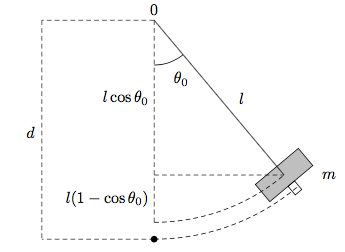
\includegraphics[scale=0.5]{schema_pendolo}


\section{Descrizione delle misure}
Attraverso il programma arduino, si sono presi i valori dei tempi di transito $t_T$ nella posizione con $\theta=0$ della bandierina di larghezza $\omega=(0.0210\pm 0.0005)m$ posta al centro ad una distanza $d=(1.16\pm0.01)m$ dal punto di rotazione del corpo e le misure del periodo T di oscillazione. Con questi dati si \'e reso possibile calcolare la velocit� media del centro di massa del corpo (posto ad una distanza $l_{CM}$) nel punto di equilibrio e, successivamente, ricavare l'ampiezza dell'oscillazione per verificare la validit� dell'equazione \eqref{eq2}. 
(Si sottolinea che il pendolo fisico pu\'o essere approssimativamente trattato come un pendolo semplice a distanza $l_{CM}$ dal punto di rotazione).

\section{Analisi Dati}
Ottenuti i dati con arduino, si \'e utilizzata la seguente equazione: $v_{o}=\frac{\omega}{t_T}\frac{l_{CM}}{d}$ per calcolare la velocit\'a del centro di massa con cui si \'e poi calcolato l'ampiezza iniziale di oscillazione $\theta_o$ con la seguente espressione: $\theta_o=\arccos(1-\frac{v_o^2}{2gl_{CM}}) $. Poi con il modulo curve-fit di  scipy.optimize di Python si \'e fatto il fit lineare con la funzione \eqref{eq2} con $\theta_o$ la variabile indipendente, il periodo T la variabile dipendente, i paremetri liberi i coefficienti  $p_1=\frac{1}{16}$, $p_2=\frac{11}{3072}$ e $l_{CM}$, senza mettere gli errori sulla T in quanto tutti uguali a 0.00007 s. Importante notare che gli errori su T non sono gaussiani, ma hanno distribuzione uniforme.

\begin{table}[!htb]
\caption{Risultato del fit lineare con curve-fit}
\label{arr1}
\centering
\[
\begin{array}{l}
\toprule
l_{CM} = (1.1266 \pm 0.0001)m \\
p_1 = 0.064 \pm 0.002  \\
p_2 = -0.022 \pm 0.027  \\
\text{Chisquare} = 11.6       \\
\text{Chisquare atteso}: 14.0 \pm 3.3  \\
\bottomrule
\end{array}
\]
\end{table}

Si nota immediatamente che a causa degli errori troppo elevati su T il coefficiente $p_2$ non pu\'o essere assolutamente ricavato attraverso questi dati in quanto troppo 'grossolani', del resto si sta cercando di rilevare un contribito di o($\theta^3$). 
Con questi valori si \'e poi realizzato un grafico della retta di best fit confrontata con i valori ottenuti per via sperimentale.


\begin{figure}[!htb]
\begin{center}
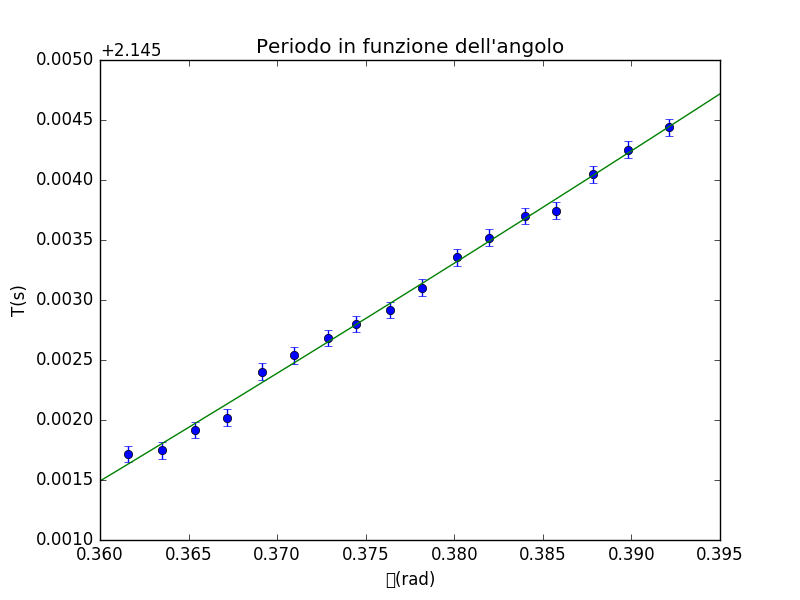
\includegraphics[width=8cm]{figura}
\end{center}
\caption{Retta di best fit (in verde) e valori sperimentali (in blu)}
\label{fig1}
\end{figure}




\section{Conclusione}
Dal test del chisquare si nota immediatamente che il chi2 ottenuto dista meno di una sigma dal valore atteso corrispondente ai gradi di libertà del problema.
Di conseguenza il p-value ricavato pari a $36$\% risulta molto buono e ci assicura che la probabilità di ottenere un vlore estremante rispetto a quello trovato è molto alta.
L'unico problema di questo fit è che a causa di errori di misura sul periodo T molto elevati, il coefficiente $p_2$ non può essere ricavato con questo fit, anche se molto buono.
\end{document}



